\documentclass[11pt]{article}
\usepackage[margin=1in]{geometry}
\usepackage{amsmath, amssymb}
\usepackage{booktabs}
\usepackage{graphicx}
\usepackage{float}
\usepackage[font=small]{caption}
\graphicspath{{../figures/}}

\title{\vspace{-1.5em}\textbf{Final Project --- Part I}\\[0.2em]
\large Numerical Methods for Ordinary Differential Equations}
\author{Hovan Boyajian \\ \small MATH 104C}
\date{Spring 2026}

\begin{document}
\maketitle

\section{Introduction}
In this project I compare several numerical methods for solving the
initial-value problem
\[
y' = f(t,y), \qquad a \le t \le b, \qquad y(a) = \alpha .
\]
The methods I implemented are Euler's method, the second-order Taylor method,
the midpoint method, the modified Euler method, Heun's third-order method, the
classical fourth-order Runge--Kutta method (RK4), the four-step
Adams--Bashforth method, and the fourth-order Adams predictor--corrector method
(whose corrector is the three-step Adams--Moulton formula). My goals are to
compare their accuracy, to see how the error behaves as the step size $h$
shrinks, to check whether the observed error matches the theoretical order of
each method, and to look at how error propagates and how stability differs from
one method to another.

All methods were coded in Python; the code is described in
Section~\ref{sec:code}. As a check, my implementations reproduce the textbook
values for Problem A to every printed digit (for example, the midpoint and Heun
columns of Tables 5.6--5.7 in the notes).

\section{The Methods}
Let $t_i = a + ih$ and let $w_i \approx y(t_i)$. The one-step methods are
\begin{align*}
\text{Euler:}\quad & w_{i+1} = w_i + h f(t_i,w_i), \\
\text{Taylor (order 2):}\quad & w_{i+1} = w_i + h f + \tfrac{h^2}{2}\,f',
   \quad f' = f_t + f_y f, \\
\text{Midpoint:}\quad & w_{i+1} = w_i + h f\!\left(t_i+\tfrac{h}{2},\,
   w_i + \tfrac{h}{2}f(t_i,w_i)\right), \\
\text{Modified Euler:}\quad & w_{i+1} = w_i + \tfrac{h}{2}
   \left[f(t_i,w_i) + f\!\left(t_{i+1}, w_i + h f(t_i,w_i)\right)\right], \\
\text{Heun (order 3):}\quad & w_{i+1} = w_i + \tfrac{h}{4}
   \left[f(t_i,w_i) + 3 f\!\left(t_i+\tfrac{2h}{3},\,
   w_i + \tfrac{2h}{3}f\!\left(t_i+\tfrac{h}{3}, w_i+\tfrac{h}{3}f(t_i,w_i)\right)\right)\right],
\end{align*}
and RK4 uses the usual four slope estimates
$k_1 = hf(t_i,w_i)$, $k_2 = hf(t_i+\tfrac h2, w_i+\tfrac{k_1}{2})$,
$k_3 = hf(t_i+\tfrac h2, w_i+\tfrac{k_2}{2})$, $k_4 = hf(t_{i+1}, w_i+k_3)$,
\[
w_{i+1} = w_i + \tfrac16(k_1 + 2k_2 + 2k_3 + k_4).
\]
The multistep methods reuse previously computed slopes. The explicit four-step
Adams--Bashforth method is
\[
w_{i+1} = w_i + \tfrac{h}{24}\left(55 f_i - 59 f_{i-1} + 37 f_{i-2} - 9 f_{i-3}\right),
\]
and the fourth-order Adams predictor--corrector method uses this formula to
predict $w_{i+1}^\ast$, then corrects once with the implicit three-step
Adams--Moulton formula
\[
w_{i+1} = w_i + \tfrac{h}{24}\left(9 f(t_{i+1}, w_{i+1}^\ast) + 19 f_i - 5 f_{i-1} + f_{i-2}\right).
\]
Because the multistep methods need the starting values $w_1, w_2, w_3$, I
generate those with RK4 before switching over, as in the textbook algorithm.
The nominal global orders are: Euler $O(h)$; Taylor, midpoint, and modified
Euler $O(h^2)$; Heun $O(h^3)$; and RK4, Adams--Bashforth, and the Adams
predictor--corrector $O(h^4)$.

\section{Problem A}
Consider
\[
y' = y - t^2 + 1, \qquad 0 \le t \le 2, \qquad y(0) = 0.5,
\]
with exact solution $y(t) = (t+1)^2 - \tfrac12 e^t$.
Table~\ref{tab:Aall} gives an overview: the maximum error of all eight methods
at $h = 0.1$, together with the observed order. Every method behaves at its
nominal order, and within an order group the leading constant still matters ---
for instance the midpoint method is about five times more accurate than the
modified Euler method even though both are order~2.

\begin{table}[H]
\centering
\caption{Problem A: maximum absolute error and observed order for all eight
methods at $h = 0.1$.}
\label{tab:Aall}
\begin{tabular}{l r r r}\hline
Method & max error ($h=0.1$) & observed order & nominal order \\
\hline
Euler & 2.42e-01 & 0.86 & 1 \\
Taylor (order 2) & 1.14e-02 & 1.89 & 2 \\
Midpoint & 3.75e-03 & 2.01 & 2 \\
Modified Euler & 1.89e-02 & 1.94 & 2 \\
Heun (order 3) & 5.73e-05 & 3.06 & 3 \\
RK4 & 6.99e-06 & 3.96 & 4 \\
Adams--Bashforth 4 & 1.85e-04 & 3.46 & 4 \\
Adams PC 4 & 1.09e-05 & 3.21 & 4 \\
\hline
\end{tabular}

\end{table}

Table~\ref{tab:Aerr} then lists the absolute error of five representative
methods at each grid point for $h = 0.2$, and Figure~\ref{fig:A} shows the
solution and the errors.

\begin{table}[H]
\centering
\caption{Problem A: absolute error at each grid point, $h = 0.2$.}
\label{tab:Aerr}
\begin{tabular}{r r rrrrr}
\hline
$t_i$ & $y(t_i)$ & Euler & Midpoint & Heun & RK4 & Adams PC \\
\hline
0.0 & 0.5000000 & 0.00e+00 & 0.00e+00 & 0.00e+00 & 0.00e+00 & 0.00e+00 \\
0.2 & 0.8292986 & 2.93e-02 & 1.30e-03 & 5.42e-05 & 5.29e-06 & 5.29e-06 \\
0.4 & 1.2140877 & 6.21e-02 & 2.73e-03 & 1.13e-04 & 1.14e-05 & 1.14e-05 \\
0.6 & 1.6489406 & 9.85e-02 & 4.28e-03 & 1.75e-04 & 1.86e-05 & 1.86e-05 \\
0.8 & 2.1272295 & 1.39e-01 & 5.95e-03 & 2.39e-04 & 2.69e-05 & 2.39e-05 \\
1.0 & 2.6408591 & 1.83e-01 & 7.69e-03 & 3.04e-04 & 3.64e-05 & 3.05e-05 \\
1.2 & 3.1799415 & 2.30e-01 & 9.48e-03 & 3.65e-04 & 4.74e-05 & 3.89e-05 \\
1.4 & 3.7324000 & 2.81e-01 & 1.12e-02 & 4.20e-04 & 5.99e-05 & 4.95e-05 \\
1.6 & 4.2834838 & 3.33e-01 & 1.29e-02 & 4.61e-04 & 7.43e-05 & 6.30e-05 \\
1.8 & 4.8151763 & 3.87e-01 & 1.42e-02 & 4.80e-04 & 9.06e-05 & 7.99e-05 \\
2.0 & 5.3054720 & 4.40e-01 & 1.51e-02 & 4.65e-04 & 1.09e-04 & 1.01e-04 \\
\hline
\end{tabular}

\end{table}

\begin{figure}[H]
\centering
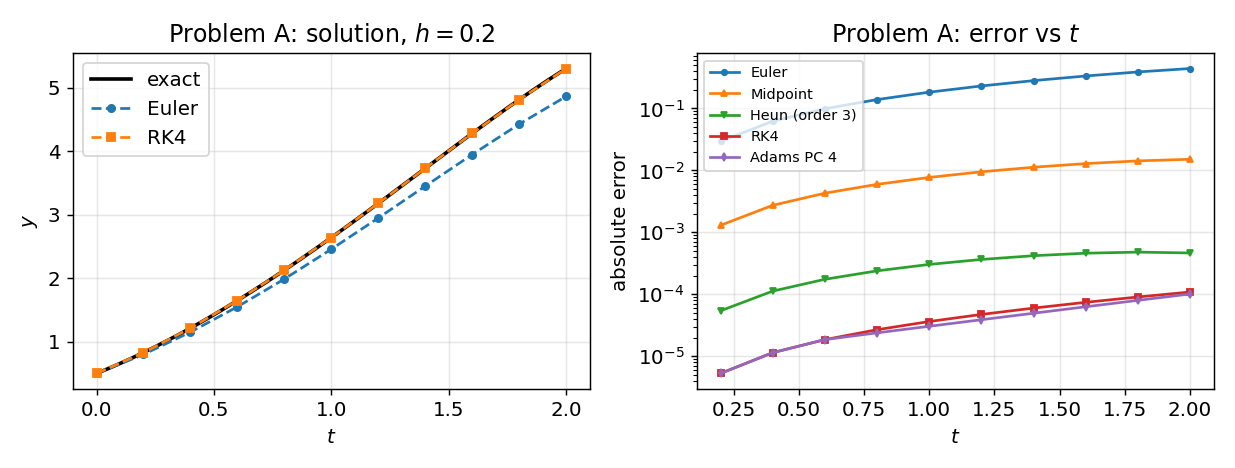
\includegraphics[width=\textwidth]{figA.png}
\caption{Problem A. Left: Euler lags the exact curve while RK4 sits on top of
it. Right: the errors separate cleanly by order --- Euler ($\sim\!10^{-1}$),
midpoint ($\sim\!10^{-2}$), Heun ($\sim\!10^{-4}$), and RK4 $\approx$ Adams PC
($\sim\!10^{-5}$).}
\label{fig:A}
\end{figure}

Euler is by far the least accurate: its error at $t=2$ is about $0.44$, while
RK4 and the Adams predictor--corrector are near $10^{-4}$, an improvement of
roughly four orders of magnitude for the same step size. To check that these
methods actually achieve their advertised order, I recomputed the maximum error
as $h$ was halved repeatedly; Table~\ref{tab:Aorder} reports the error and the
observed order $\log_2(e_{2h}/e_h)$.

\begin{table}[H]
\centering
\caption{Problem A: maximum absolute error and observed order (in parentheses)
as $h$ is halved.}
\label{tab:Aorder}
\begin{tabular}{r rrrrr}
\hline
$h$ & Euler & Midpoint & Heun & RK4 & Adams PC \\
\hline
0.2000 & 4.40e-01 (--) & 1.51e-02 (--) & 4.80e-04 (--) & 1.09e-04 (--) & 1.01e-04 (--) \\
0.1000 & 2.42e-01 (0.86) & 3.75e-03 (2.01) & 5.73e-05 (3.06) & 6.99e-06 (3.96) & 1.09e-05 (3.21) \\
0.0500 & 1.27e-01 (0.92) & 9.28e-04 (2.01) & 7.01e-06 (3.03) & 4.42e-07 (3.98) & 9.13e-07 (3.58) \\
0.0250 & 6.55e-02 (0.96) & 2.30e-04 (2.01) & 8.66e-07 (3.02) & 2.78e-08 (3.99) & 6.60e-08 (3.79) \\
0.0125 & 3.32e-02 (0.98) & 5.74e-05 (2.01) & 1.08e-07 (3.01) & 1.74e-09 (4.00) & 4.43e-09 (3.90) \\
\hline
\end{tabular}

\end{table}

The observed orders settle down to $1, 2, 3, 4$ for Euler, midpoint, Heun, and
RK4 respectively, matching the theoretical local-truncation-error analysis. The
Adams predictor--corrector approaches order $4$ as well; it starts a little
below $4$ on the coarsest grids because of the RK4 start-up values and then
improves as $h$ shrinks.

\section{Problem B}
Consider
\[
y' = 2y, \qquad 0 \le t \le 2, \qquad y(0) = 1,
\]
with exact solution $y(t) = e^{2t}$. This solution grows exponentially, which
makes it a good test of how error propagates. Table~\ref{tab:Berr} compares
Euler and RK4 at $h = 0.1$.

\begin{table}[H]
\centering
\caption{Problem B: exponential growth, $h = 0.1$.}
\label{tab:Berr}
\begin{tabular}{r r r r r}\hline
$t_i$ & $y(t_i)$ & Euler & Euler error & RK4 error \\
\hline
0.0 & 1.000000 & 1.000000 & 0.000000 & 0.00e+00 \\
0.2 & 1.491825 & 1.440000 & 0.051825 & 6.74e-06 \\
0.4 & 2.225541 & 2.073600 & 0.151941 & 2.01e-05 \\
0.6 & 3.320117 & 2.985984 & 0.334133 & 4.50e-05 \\
0.8 & 4.953032 & 4.299817 & 0.653215 & 8.95e-05 \\
1.0 & 7.389056 & 6.191736 & 1.197320 & 1.67e-04 \\
1.2 & 11.023176 & 8.916100 & 2.107076 & 2.99e-04 \\
1.4 & 16.444647 & 12.839185 & 3.605462 & 5.20e-04 \\
1.6 & 24.532530 & 18.488426 & 6.044104 & 8.86e-04 \\
1.8 & 36.598234 & 26.623333 & 9.974901 & 1.49e-03 \\
2.0 & 54.598150 & 38.337600 & 16.260550 & 2.47e-03 \\
\hline
\end{tabular}

\end{table}

\begin{figure}[H]
\centering
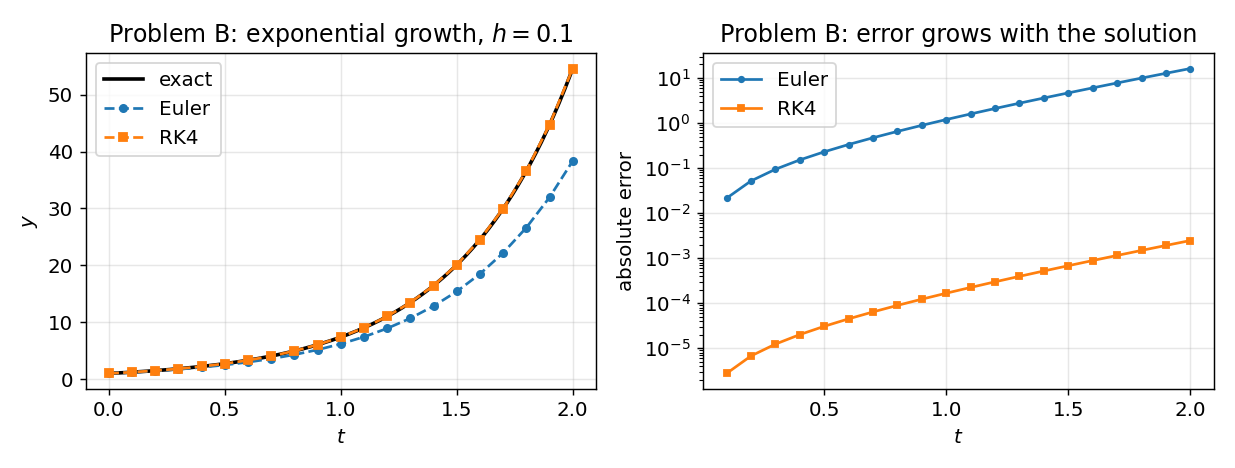
\includegraphics[width=\textwidth]{figB.png}
\caption{Problem B. The Euler error grows right along with the solution, while
RK4 stays accurate. Note the logarithmic scale on the right.}
\label{fig:B}
\end{figure}

The Euler error grows from about $0.05$ at $t = 0.2$ to over $16$ at $t = 2$.
This is exactly what error propagation predicts: when $y' = 2y$, the factor
$f_y = 2 > 0$ amplifies any existing error at every step, so the global error
itself grows roughly like $e^{2t}$. RK4 keeps the error near $10^{-3}$ over the
whole interval --- a higher-order method is much better at keeping the
propagated error small, but the underlying growth of the problem is still
visible in the slow climb of the RK4 error curve.

\section{Problem C (student-designed)}
For my own problem I chose
\[
y' = -10y + \sin t, \qquad 0 \le t \le 3, \qquad y(0) = 1,
\]
with exact solution
\[
y(t) = \frac{10\sin t - \cos t}{101} + \frac{102}{101}\,e^{-10t}.
\]
I picked this because the $-10y$ term causes a rapid initial decay (a mild
``stiffness''), which is exactly the situation where explicit methods can run
into trouble if the step size is too large. Table~\ref{tab:Cstable} shows the
maximum error of each method at the stable step $h = 0.1$.

\begin{table}[H]
\centering
\caption{Problem C: maximum absolute error at $h = 0.1$.}
\label{tab:Cstable}
\begin{tabular}{l r r}\hline
Method & max error ($h=0.1$) & order \\
\hline
Euler & 3.72e-01 & 1 \\
Midpoint & 1.33e-01 & 2 \\
Heun & 3.49e-02 & 3 \\
RK4 & 7.19e-03 & 4 \\
Adams PC & 2.42e-02 & 4 \\
\hline
\end{tabular}

\end{table}

\begin{figure}[H]
\centering
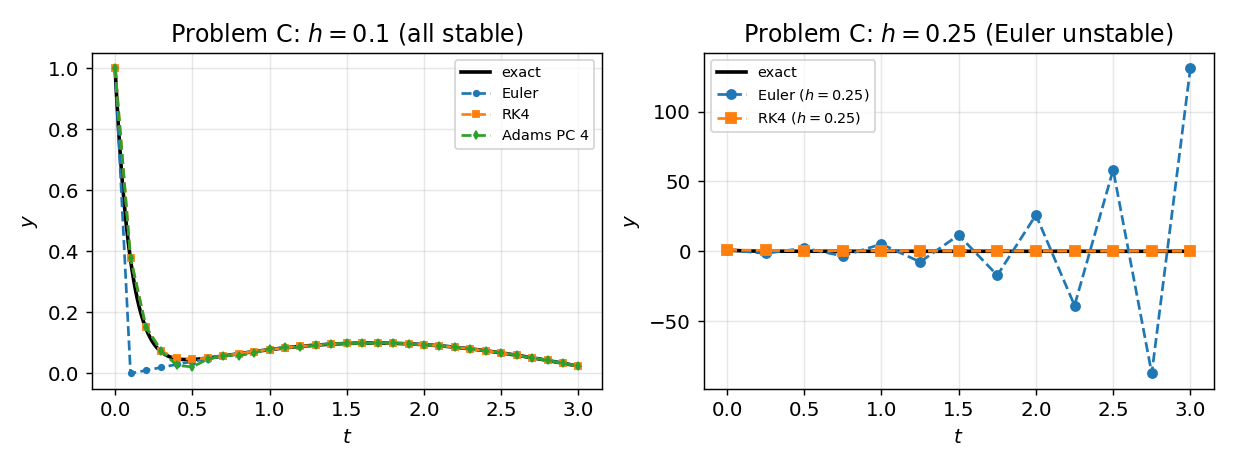
\includegraphics[width=\textwidth]{figC.png}
\caption{Problem C. Left: at $h = 0.1$ every method tracks the exact solution
(Euler is slightly rough through the sharp initial decay). Right: at $h = 0.25$
Euler is outside its stability region and oscillates with growing amplitude,
while RK4 --- which has a larger stability region --- stays accurate.}
\label{fig:C}
\end{figure}

Even at the stable step the errors here are larger than in Problem A, because
the steep transient near $t = 0$ is hard to resolve; the largest error for
every method occurs in that region. The stability difference shows up clearly
when I enlarge the step. For Euler, stability on this problem requires
$-2 < h\lambda < 0$ with $\lambda = -10$, i.e. $h < 0.2$. At $h = 0.25$ this is
violated: Euler oscillates and blows up to $w(3) \approx 131$ even though the
true solution is about $0.024$. RK4 has a larger real-axis stability region and
remains stable at $h = 0.25$ ($w(3) \approx 0.028$). Pushing further to
$h = 0.3$ eventually destabilizes RK4 too, which confirms that explicit methods
trade a larger stability region for more work per step but never have an
unbounded one.

\section{Discussion}
\textbf{Which methods are most accurate?} For a fixed step size, accuracy tracks
the order of the method. RK4 and the Adams predictor--corrector (both order 4)
were the most accurate in every experiment, followed by Heun (order 3), the
order-2 methods, and finally Euler.

\textbf{How does decreasing $h$ affect the error?} Each time $h$ is halved, the
error drops by a factor of about $2^p$, where $p$ is the order
(Table~\ref{tab:Aorder}): roughly $2\times$ for Euler, $4\times$ for the
order-2 methods, $8\times$ for Heun, and $16\times$ for RK4.

\textbf{Does the observed error agree with the theory?} Yes. The measured orders
in Table~\ref{tab:Aorder} converge to the predicted $1, 2, 3, 4$, which is the
clearest confirmation that the implementations are correct and that the
truncation-error analysis describes the real behavior.

\textbf{Why does RK4 usually beat Euler?} Euler uses only the slope at the
left endpoint, so it commits an $O(h^2)$ error every step. RK4 samples the slope
four times per step and combines them so that error terms through $h^4$ cancel,
giving local error $O(h^5)$ and global error $O(h^4)$. It costs four function
evaluations per step instead of one, but the accuracy gain is enormous.

\textbf{Why can methods of the same order behave differently?} The midpoint and
modified Euler methods are both order 2, yet on Problem A the midpoint method
was about five times more accurate (Table~\ref{tab:Aall}). They have the same
order but different leading error constants, so
``same order'' only means the errors shrink at the same \emph{rate}, not that
they are the same size. The same is true of RK4 versus the Adams
predictor--corrector: both order 4, but with slightly different constants.

\textbf{How does error propagate over time?} On Problem A and especially Problem
B the error grows as $t$ increases, because each step's new error is carried
forward and, when $f_y > 0$, amplified. On Problem C, where $f_y = -10 < 0$, the
exact dynamics instead damp errors --- as long as the method is stable.

\textbf{Which methods appear more stable?} For a fixed step size the higher-order
Runge--Kutta methods have larger stability regions, so RK4 tolerated a step
($h = 0.25$) on Problem C that made Euler blow up. But no explicit method is
unconditionally stable: a large enough step destabilizes all of them.

\section{Code}
\label{sec:code}
All methods are implemented in \texttt{ode\_methods.py}, and
\texttt{run\_project.py} reproduces every figure and table in this report;
\texttt{check\_regression.py} verifies the output against the published
textbook values. The code is available at:

\begin{center}
\texttt{https://github.com/<your-username>/math104c-final-project-1}
\end{center}

\end{document}
